\documentclass[onecolumn, draftclsnofoot,10pt, compsoc]{IEEEtran}
\usepackage{graphicx}
\usepackage{url}
\usepackage{setspace}
\usepackage{longtable}

\usepackage{geometry}
\geometry{textheight=9.5in, textwidth=7in}

% 1. Fill in these details
\def \CapstoneTeamName{		}
\def \CapstoneTeamNumber{		6}
\def \GroupMemberOne{			Donghao Lin}
\def \GroupMemberTwo{			Joshua Diedrich}
\def \GroupMemberThree{			Christopher Breniser}
\def \CapstoneProjectName{		Race Car Scanning and Modeling}
\def \CapstoneSponsorCompany{	REHV}
\def \CapstoneSponsorPersonOne{	Kyson Montague}
\def \CapstoneSponsorPersonTwo{	Rodney Stauber}

% 2. Uncomment the appropriate line below so that the document type works
\def \DocType{	
				%Requirements Document
				%Technology Review
				%Design Document
				Progress Report
				}
			
\newcommand{\NameSigPair}[1]{\par
\makebox[2.75in][r]{#1} \hfil 	\makebox[3.25in]{\makebox[2.25in]{\hrulefill} \hfill		\makebox[.75in]{\hrulefill}}
\par\vspace{-12pt} \textit{\tiny\noindent
\makebox[2.75in]{} \hfil		\makebox[3.25in]{\makebox[2.25in][r]{Signature} \hfill	\makebox[.75in][r]{Date}}}}
% 3. If the document is not to be signed, uncomment the RENEWcommand below
%\renewcommand{\NameSigPair}[1]{#1}

%%%%%%%%%%%%%%%%%%%%%%%%%%%%%%%%%%%%%%%
\begin{document}
\begin{titlepage}
    \pagenumbering{gobble}
    \begin{singlespace}
    	
\includegraphics[height=4cm]{coe_v_spot1}
        \hfill 
        % 4. If you have a logo, use this includegraphics command to put it on the coversheet.
        %\includegraphics[height=4cm]{CompanyLogo}   
        \par\vspace{.2in}
        \centering
        \scshape{
            \huge CS Capstone \DocType \par
            {\large\today}\par
            \vspace{.5in}
            \textbf{\Huge\CapstoneProjectName}\par
            \vfill
            {\large Prepared for}\par
            \Huge \CapstoneSponsorCompany\par
            \vspace{5pt}
            {\Large\NameSigPair{\CapstoneSponsorPersonOne}\par}
            {\Large\NameSigPair{\CapstoneSponsorPersonTwo}\par}
            {\large Prepared by }\par
            Group\CapstoneTeamNumber\par
            % 5. comment out the line below this one if you do not wish to name your team
            \CapstoneTeamName\par 
            \vspace{5pt}
            {\Large
                \NameSigPair{\GroupMemberOne}\par
                \NameSigPair{\GroupMemberTwo}\par
                \NameSigPair{\GroupMemberThree}\par
            }
            \vspace{20pt}
        }
        \begin{abstract}
        % 6. Fill in your abstract    
        	This document describes the method used to measure the axle length of Indie Lights race cars using single image distance scanning. This document will explore various OpenCV libraries and functions used, as well as the formulas used to calculate Indie Lights race cars axle length.
        \end{abstract}     
    \end{singlespace}
\end{titlepage}
\newpage
\pagenumbering{arabic}
\tableofcontents
% 7. uncomment this (if applicable). Consider adding a page break.
%\listoffigures
%\listoftables
\clearpage

\section{Purpose/Goals}
Our project is based around the idea of supplementing a process that Race Cars undergo before each race, referred to as a pre race inspection.  Specifically, our project works on a car called an Indy Light.  An Indy Light is a certain type of race car, similar to that of an Indy Car.  Prior to each race, every Indy Light car must meet certain requirements to pass inspection.  These requirements include things like weight, width, tire pressure, wing angle, and many more.  An inspection starts with the vehicle being rolled onto a scale.  Next, the inspection team takes each required measurement of the car by hand, using special tooling.  The car then either passes or fails it’s inspection.
\newline

\noindent The purpose of our project is to supplement the pre race inspection process using automated technology.  It takes a lot of manpower, and tedious work to make each measurement on the car.  Having people manually using tools to make every measurement makes for a somewhat slow inspection.  Our project aims at replacing some of these manual measurements with automated ones.  This should reduce the man-power needed to obtain measurements, and make it as easy as clicking a button.  Our device should also add to the process by measuring a few things that the team is not already picking up.
\newline

\noindent The first measurements we want to make are called camber and toe.  These relate to the wheels of the vehicle, specifically their angle.  Wheels are not all pointed straight forward and straight up and down, they often have some angle associated with them. Camber is the vertical angle of the wheel, while toe is the horizontal angle of the wheel.
\newline

\noindent Next we want to measure the wheelbase of the car.  The wheelbase is the distance from the center axle of the front wheels to the center axle of the back wheels.
\newline

\noindent Finally,  we want to measure what is called the track.  Track is basically the width of the car.  It is the distance horizontally from wheel to wheel.  This measurement is especially difficult to take by hand, because you can't just spread a measuring tape from one wheel across the car to the other.
\newline

\noindent The measurements we are taking are going to be very important.  Inspection for each car can actually stop that car from competing in the race, which is a big deal for the driver or company associated with that car.  Because of that, our system needs to meet some strict goals when it comes to consistency and accuracy.  One goal is that our design is cost efficient.  We want to aim to use the least amount of expensive equipment without affecting the accuracy of our measurements too much.  Our client can allow us some spending, but we can’t be purchasing top of the line equipment to create our product.  Our next goal is save time.  One of the main points of our project is to save the inspection team time.  They have a lot of measurements to get through during an inspection, and we want to cut down on the time it takes to make those.  Precision and accuracy is likely our most important goal.  The system needs to take measurements that are accurate and consistent enough for our system to be considered reliable.  Without reliability, our system could not be trusted to pass or fail a car.  If our system is inconsistent enough that it has to be double checked each time, then there is no point having it at all.  Finally, the system needs to be fast and repetitive.  Each car is measured is a matter of minutes, and then the next one is rolled up onto the scale.  The system has to have short enough downtime that it is able to repeat it’s measuring process over and over again during that short time period.

\newline

\noindent The measurements laid out earlier are a bare minimum requirement that we want to reach.  Through discussion with our client, we have also created some stretch goals that we might eventually want to add.  One possible stretch goal is to obtain a measurement on the wing angle.  This is currently a measurement done by hand, but with some additions, it would be possible to obtain.  Another stretch goal that we wish to achieve is some sort of user interface that implements a rough outline of an Indy Light car.  We expect this user interface to have a contoured layout of the Indy Light being measured, with labels on it for each of the measurements taken.  This could be held by one of the employees on a mobile device or pad, and would allow for easy viewing on the vehicle.

\section{Current Progress}
The current progress of the project can be divided into three sections.  Image detection, depth measurements, and post depth calculations.

\subsection{Image Detection}
Our project implements a number of OpenCV libraries to accommodate the image detection for our fiducials.  We use algorithms like Canny for edge detection in order to find a number of 90 degree corners throughout the program.  This section of our project is responsible for locating all the squares in a photo and finding the center point of each of them.  It then does some arithmetic on the x,y locations of the points to find which point is the center, right, left, top, and bottom.  At our current alpha build the functionality for this part of our program is fairly accurate in good lighting and high contrast squares.  The figure below shows an image being ran through the program and the key points highlighted by black dots.

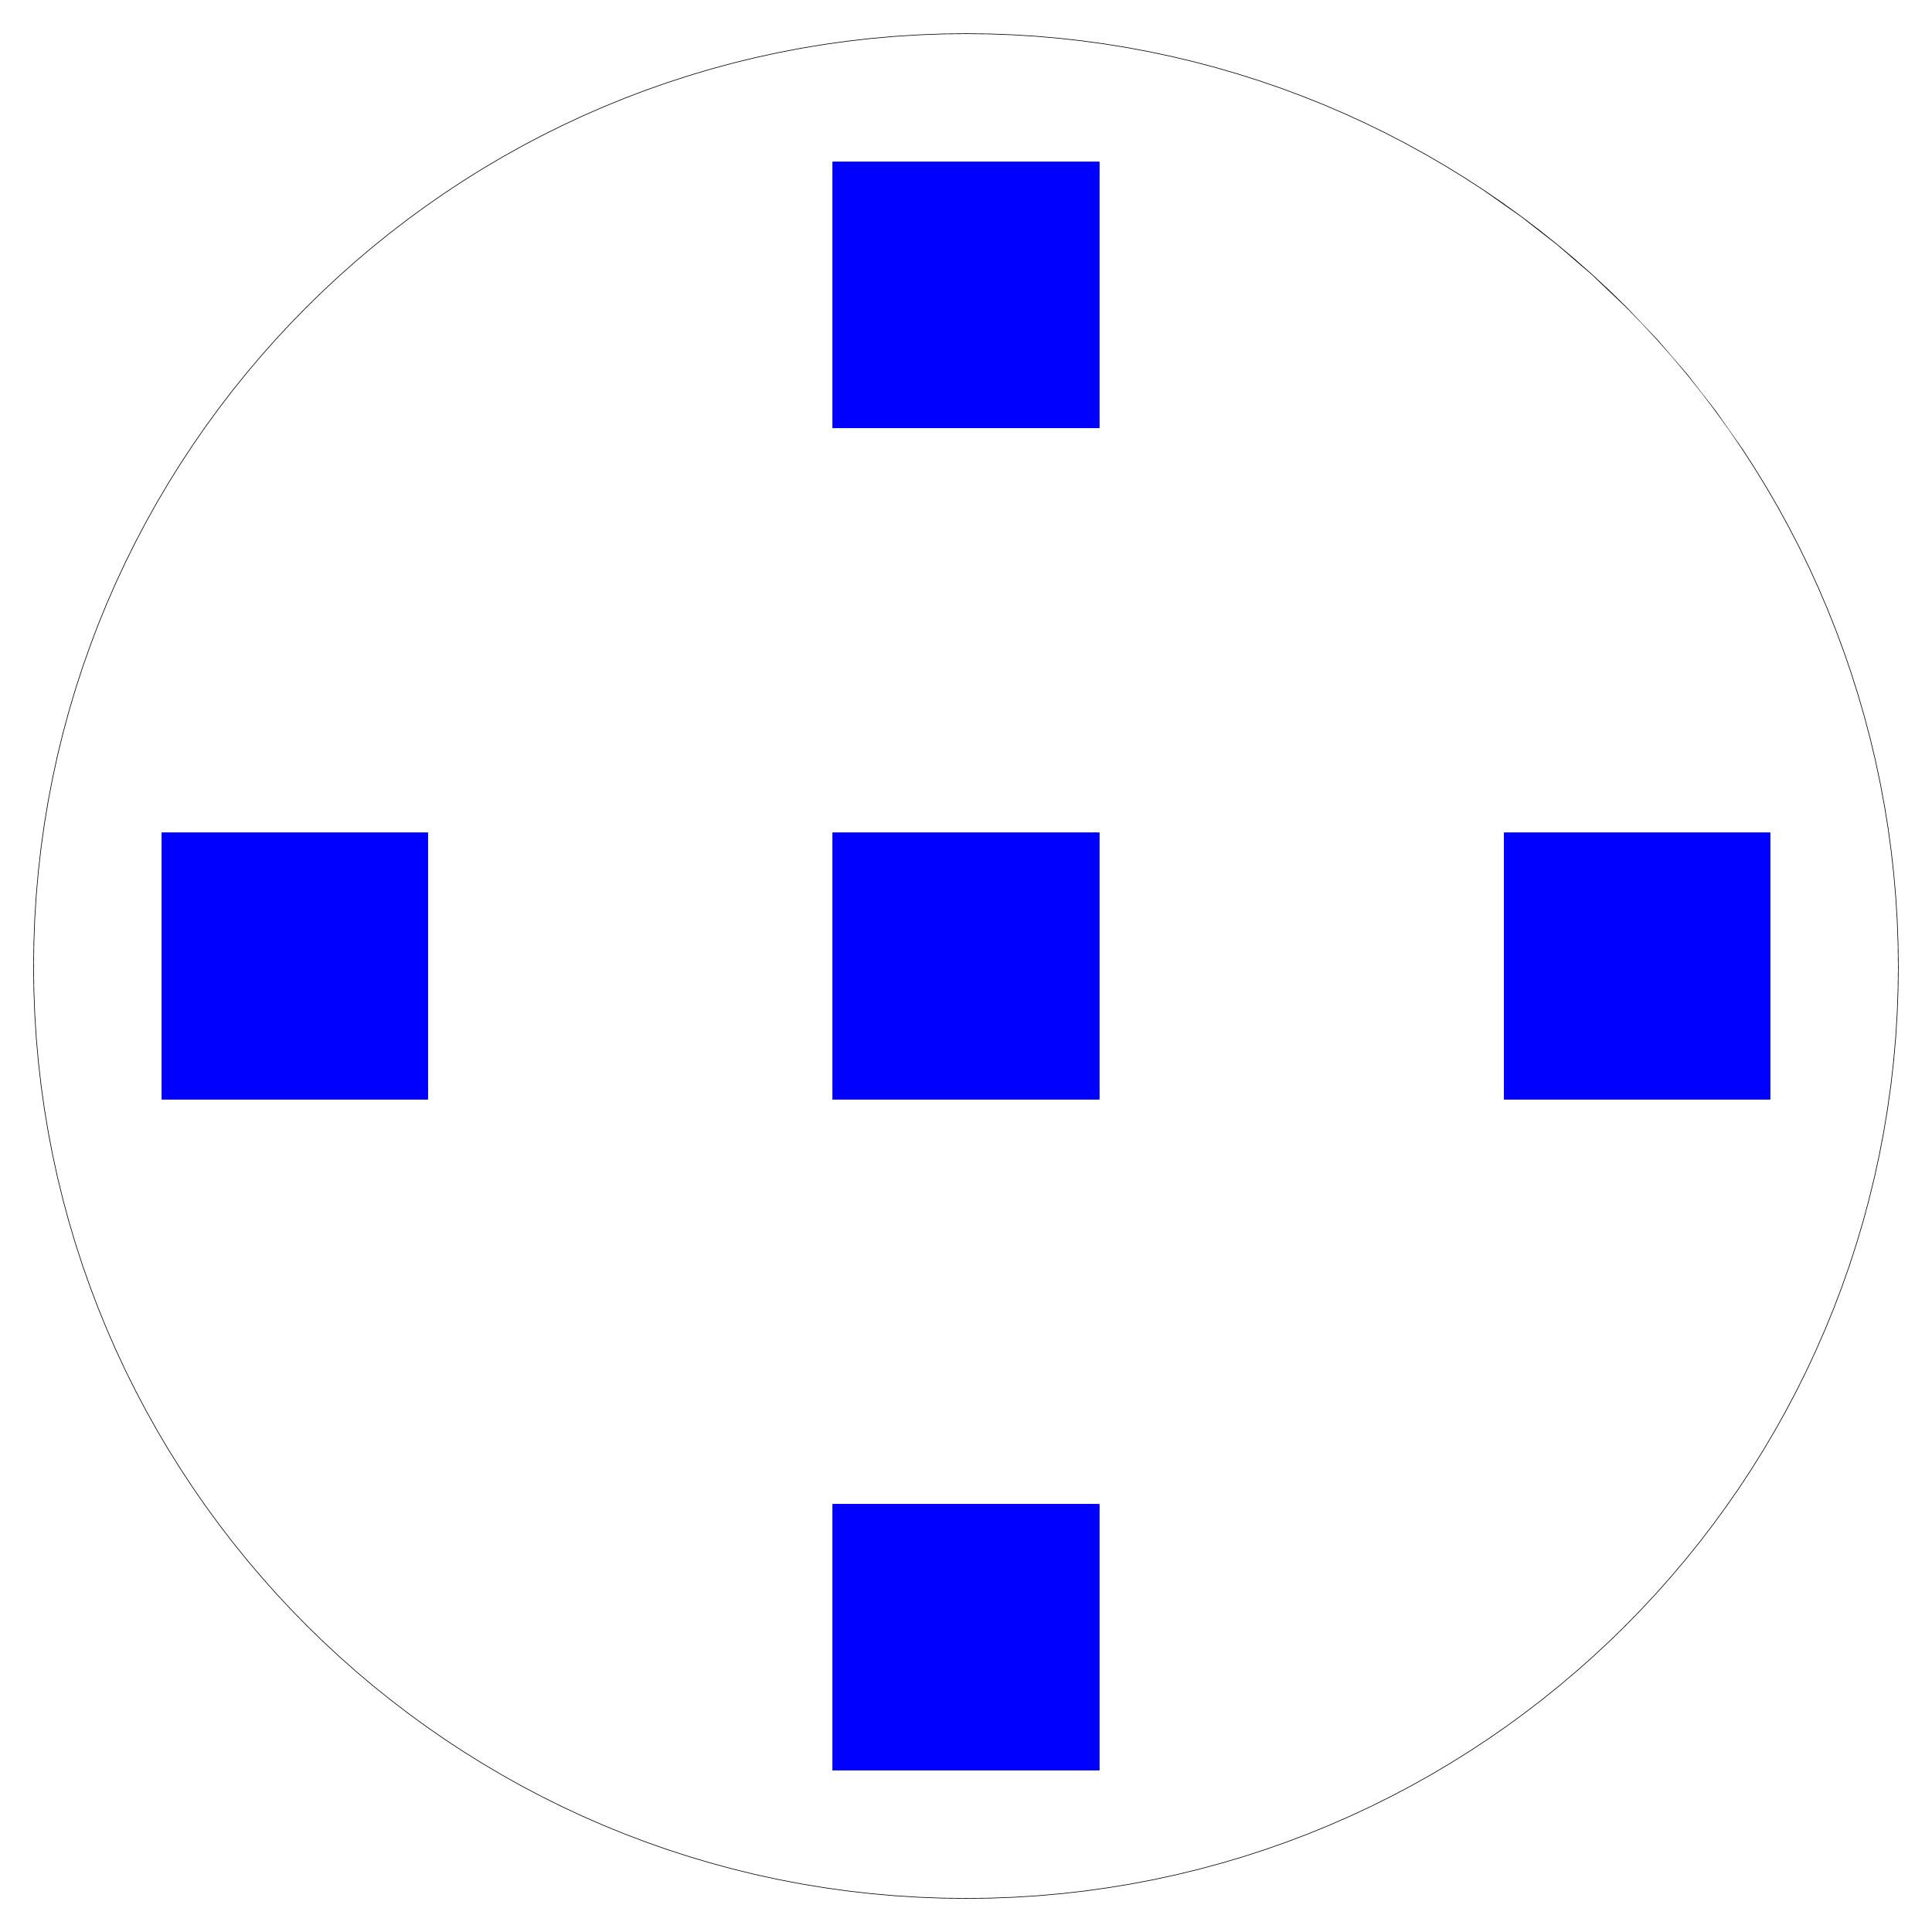
\includegraphics[width=5cm, height=5cm]{images/alphafiducial.jpg}
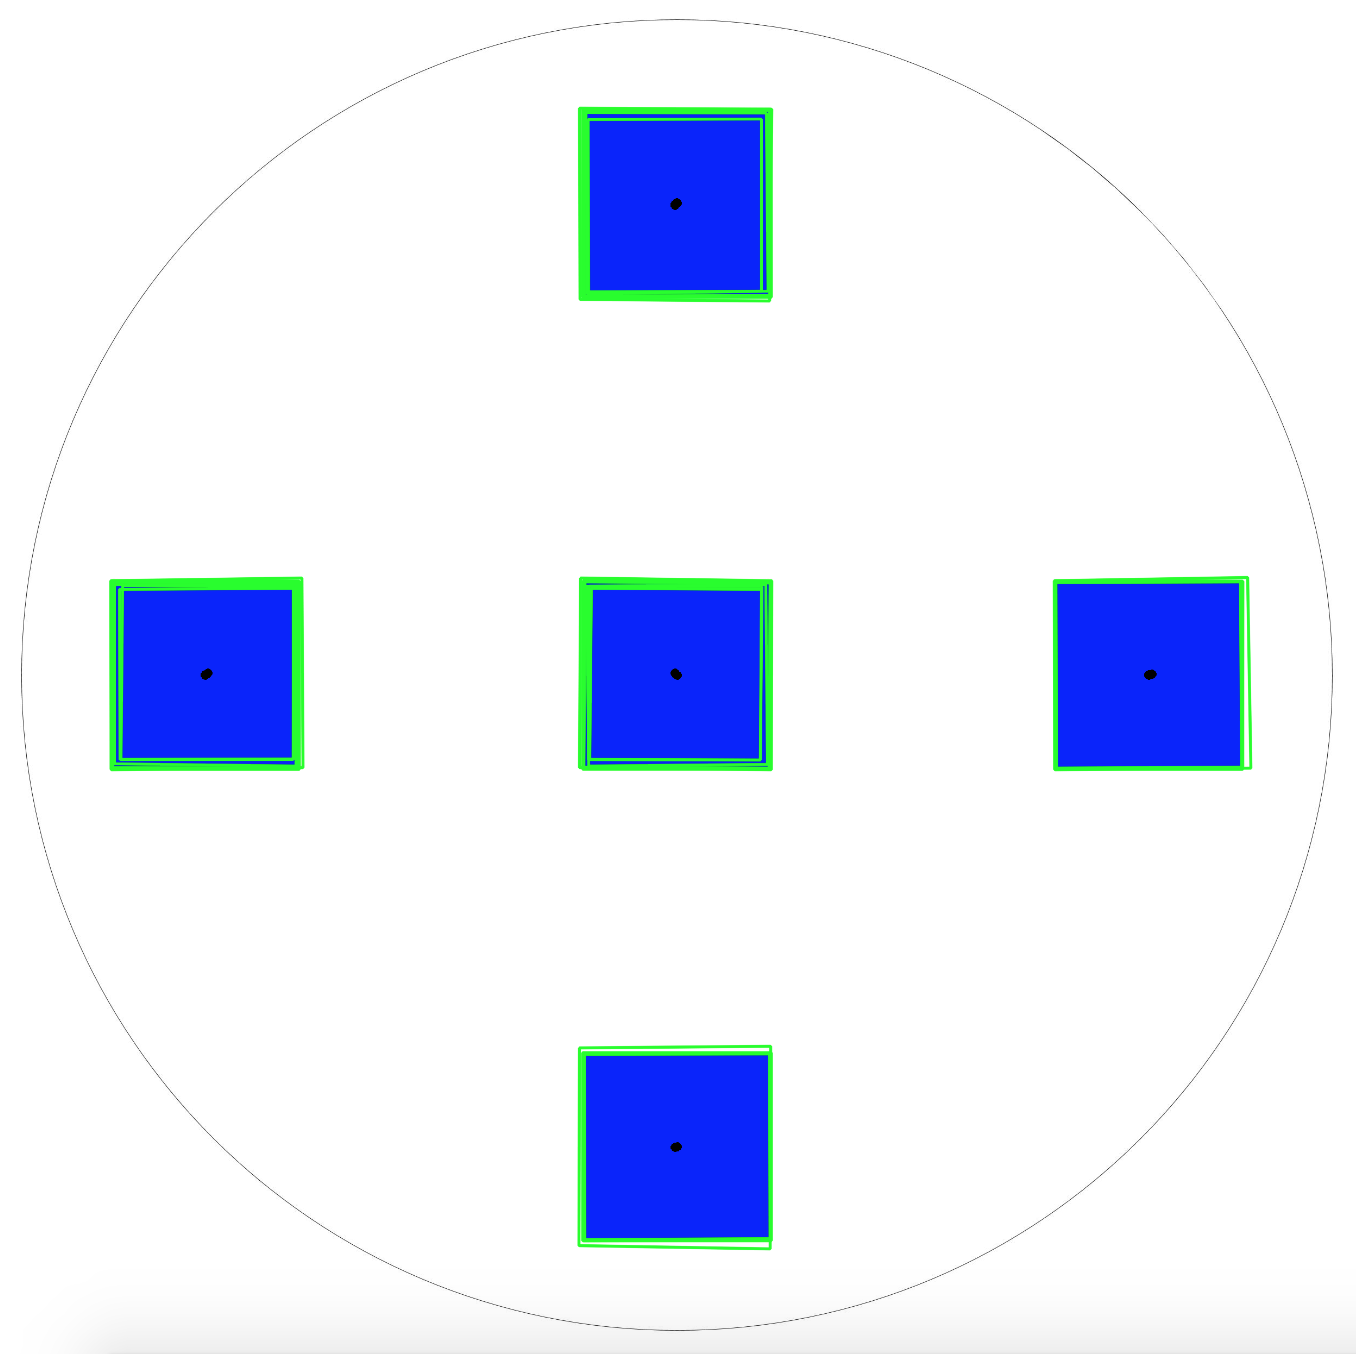
\includegraphics[width=5cm, height=5cm]{images/marked.png}

\subsection{Depth Measurements}
We are using a ZED camera to make our depth measurements.  This works down to a millimeter accuracy in good lighting on an NVIDIA GPU with compute capability of 3.0 or greater.  The software being used for this section is from the ZED SDK libraries.  This section of our alpha build can correctly measure the depth of a pixel in the x,y,z plane from the left eye of the lens with fair accuracy.  The below image is an example of the output from our ZED Camera.

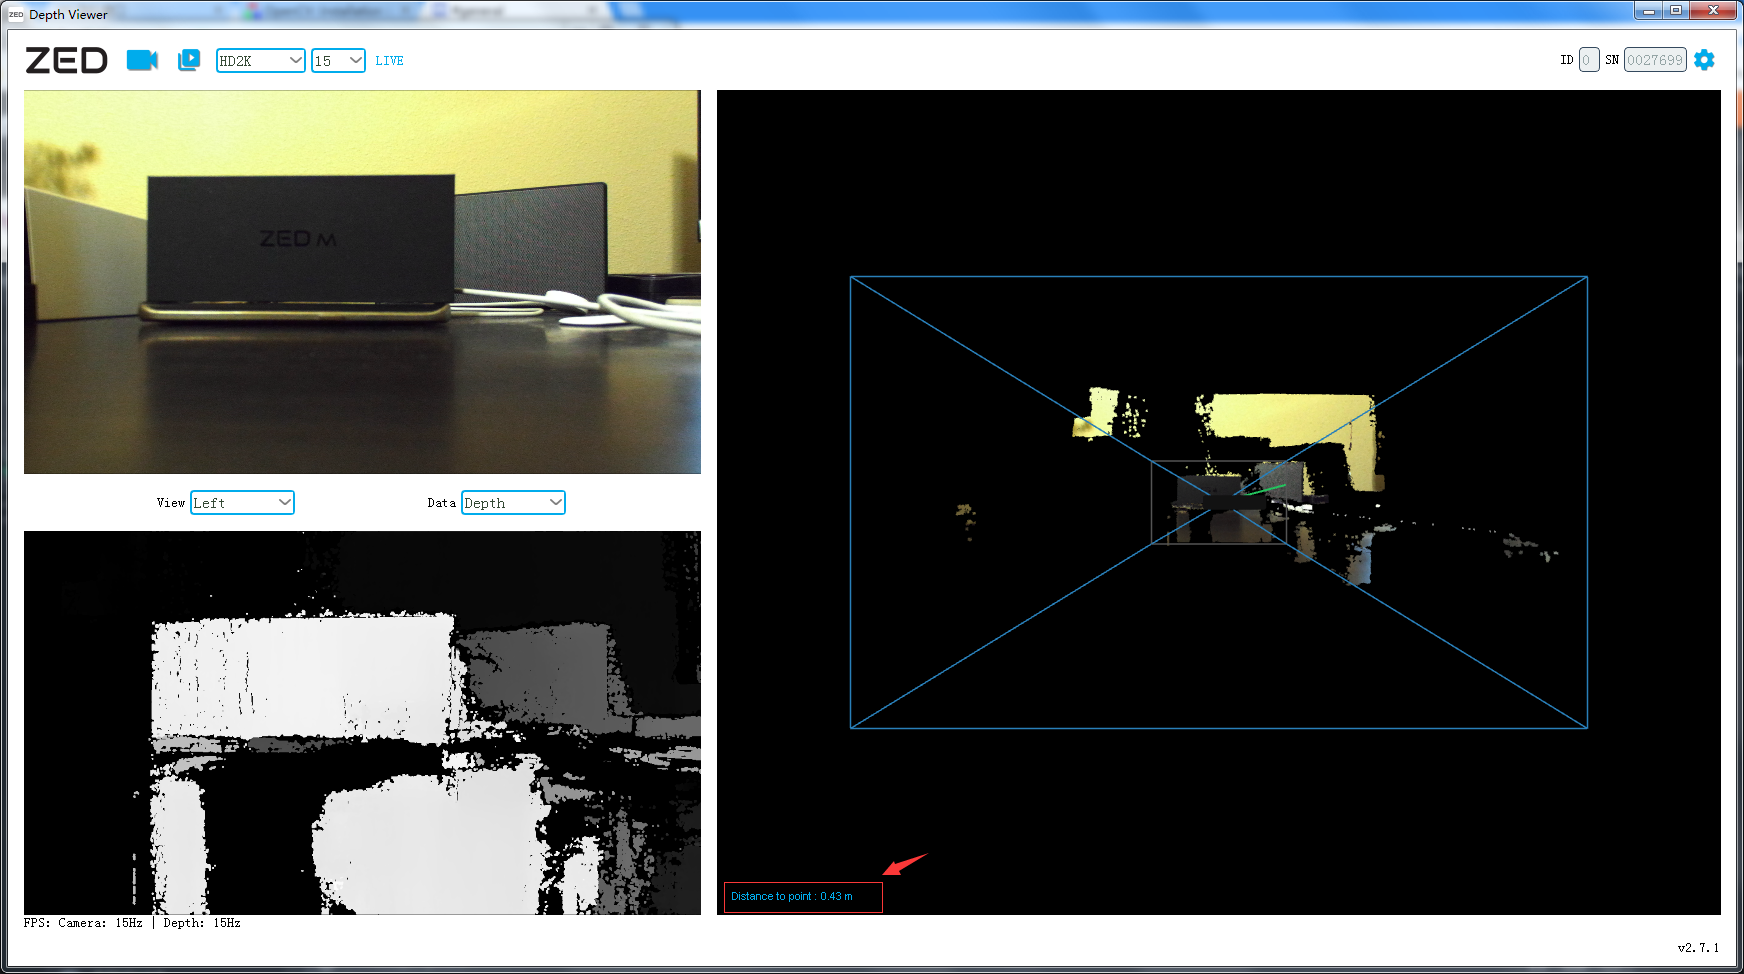
\includegraphics[width=8cm, height=5cm]{images/ZED.png}

\subsection{Post Measurements}
The alpha build includes libraries to accommodate our measurements once they are taken.  These calculations are responsible for calculating the track, axle width, Camber, and Tow.


\section{To-Do's}
All of our alpha software works independently of one another.  They do not yet share information with each other.  Our next step for the beta build is to share the output of each separate part of our program with one another.  This will involve sending the pixel outputs from the image detection to the ZED camera portion, then sending the depth measurements from the ZED cameras to the post measurements portion.  This should tie our whole system together and allow us to make measurements.

\subsection{Fiducials}
Currently our system looks at fiducials that are generated solely with software on Google Drawings.  For our next build the goal is to have a physical fiducial similar to the one that we will be bolting onto the wheel of the Indy Lights Cars.

\subsection{User Interface}
Our alpha user interface consists of executing a Linux command generates when our code is compiled.  The beta build will have to clean up this UI and compile our program with one Make command.

\section{Obstacles} The various obstacles we overcame this term so far were somethings we expected, but in the end had better outcomes that first imagined. For example, within the first week of this term we were fresh off researching new ideas using stereo vision and were ready to tackle the various measurement we had in mine. However, we were unable to reliably zero in the location of the car body. After meeting with our client, we confirmed that the location of the vehicle will be close enough to zero that we can proceed without concerning ourselves with the car frame itself. 
\newline

\noindent The majority of this term we were faced with the challenge of learning the new technology we transitioned to. This took up a considerable about of time as we were starting from fresh. Our solution throughout this term, though very predictable, has been researching proper use of opencv and understanding the math behind creating a depth map. However once we received a Zed Mini stereo camera, we were able to use Zed Minis sdk and libraries to forgo the process of creating depth maps manually. This allowed us to focus on creating a wrapper that will use our opencv software with existing Nvidia libraries to measure the base information we need to input into our calculation functions. The only outstanding obstacle we face, other than further testing and research, is ensuring that the hardware we are using our software on includes an Nvidia graphics card. At this point we have been doing all testing on desktops in our homes, which has been a hamper on team based testing. The solution to this is to acquire an external GPU to use with our laptops during development.

\section{Retrospective}
\begin{longtable}{ | p{0.075\linewidth} | p{0.3\linewidth} | p{0.3\linewidth} | p{0.3\linewidth} |} \hline
Weeks & Started & Continued & Actions  \\ \hline
1 & Setup meeting time with client for the following week. & Continued research about stereo vision started over winter break. & Setup regular meeting time for group and TA. \\ \hline
2 & Gathering a better understanding on our requirements from TA after our stereo vision adjustment. & Researching opencv to use with depth maps. Researching the manual acquisition of a depth map using two cameras. & Narrowed down previously established goals to essentials. \\ \hline
3 & Elevator pitch and poster draft. 
Developing code for fiducial acquisition using opencv in c++.
 & Research on depth map generation. Making alterations to our poster to prepare for next week’s poster review. & Practised our elevator pitch. 
Got a better understanding of presenting to different demographics. \\ \hline
4 & None. & Poster alterations, code research on depth maps, developing opencv and fiducial capturing. & Poster review was delayed due to inclement weather. Setup time for next week. \\ \hline
5 & Poster review gave us good feedback to take our layout and presentation. Started redesign draft. & Further code development for opencv and fiducial acquisition. Finding outline consistently. Need to work on finding center next. & Reached out to Kevin about stereo camera and answered some rudimentary questions. \\ \hline
6 & Started code base for Zed camera in a separate library. & Testing code to acquire fiducials on imputed images. Consistently finding centers on photos we tested.  & Acquired Zed mini stereo camera. Finished alpha level libraries for calculations and opencv libraries. Zed camera removed the need to manually create depth maps. \\ \hline
7 & At home testing of Zed mini. (required Nvidia GPU). & More in depth testing on fiducials and center-of-square locating. 
Testing sdk software wrapper for Zed mini. & TA instructed us to reach out to kevin about acquiring a GPU dock for developing on our laptops. \\ \hline
\end{longtable}

\end{document}